\documentclass{article}
\usepackage[margin=3pt,landscape]{geometry}
\usepackage[utf8]{inputenc}
\usepackage[T1]{fontenc}
\usepackage{multicol}
\usepackage{amsmath}
\usepackage{amssymb}
\usepackage{stmaryrd}
\usepackage{fixltx2e}
\usepackage{textcomp}
\usepackage{graphicx}
\usepackage{epstopdf}
\usepackage{wrapfig}
\usepackage{picinpar}
\usepackage{amsfonts}
\usepackage{ upgreek }

%\usepackage[nopar]{lipsum}%just to generate text for the example

% redefinition of \normalsize to use \footnotesize and decrease the values for
% \abovedisplyskip, \belowdisplayskip, and the "short" variants
\makeatletter
\renewcommand\normalsize{%
  \@setfontsize\footnotesize\@viiipt{8.8}%
   \abovedisplayskip 1\p@ \@plus\p@ \@minus\p@
   \belowdisplayskip 1\p@ \@plus\p@ \@minus\p@
   \abovedisplayshortskip \z@ \@plus\p@
   \belowdisplayshortskip \z@ \@plus\p@ \@minus\p@
   \let\@listi\@listI}
\makeatother

\pagestyle{empty}

% multicol parameters
\setlength\premulticols{1pt}
\setlength\postmulticols{1pt}
\setlength\multicolsep{1pt}
\setlength\columnsep{2pt}
\raggedright

% For the source codes
\usepackage{stackengine}
\usepackage{listings}
\lstdefinestyle{customc}{
  belowcaptionskip=1\baselineskip,
  breaklines=true,
%  frame=L,
%  xleftmargin=\parindent,
  xleftmargin=0pt,
  language=C,
  showstringspaces=false,
  basicstyle=\tiny\ttfamily,
  tabsize=1,
%  numbersep=8pt,
%  numbers=left,
%  xleftmargin=0.5cm,
  frame=tlbr,
%  framesep=2pt,
  framerule=0pt
}

\lstset{escapechar=@,style=customc}

% For Math Alphabet
\DeclareMathAlphabet{\pazocal}{OMS}{zplm}{m}{n}
\newcommand{\Kb}{\pazocal{K}}
\newcommand{\Ib}{\pazocal{I}}
\newcommand{\Sb}{\pazocal{S}}
\newcommand{\Rb}{\pazocal{R}}
\newcommand{\Ub}{\pazocal{U}}
\newcommand{\Lb}{\pazocal{L}}
\newcommand{\Hb}{\pazocal{H}}
\newcommand{\Bb}{\pazocal{B}}
\newcommand{\Vb}{\pazocal{V}}
\newcommand{\Qb}{\pazocal{Q}}
\newcommand{\Ab}{\pazocal{A}}
\newcommand{\Fb}{\pazocal{F}}
\newcommand{\Db}{\mathfrak{D}}
\graphicspath{{./Pictures/}}

\begin{document}
\begin{multicols}{4}
\textbf{Propositional Logic Syntactic Sugar} 
\begin{gather*} 
{\varphi \Leftrightarrow \psi := (\neg \varphi \vee \psi) \wedge (\neg \psi \vee \varphi)} \qquad {\varphi \rightarrow \psi := \neg \varphi \vee \psi} \\
{\varphi \oplus \psi := (\varphi \wedge \neg \psi) \vee (\psi \wedge \neg \varphi) }\qquad {\varphi \barwedge \psi := \neg (\varphi \wedge \psi)} \\
{(\alpha \Rightarrow \beta | \gamma) := ( \neg \alpha \vee \beta) \wedge (\alpha \vee \gamma)} \quad {\varphi \bar{\vee}\psi := \neg (\varphi \vee \psi)}
\end{gather*}
\textbf{Distributivity:} ${a \wedge ( b \vee c ) = (a \wedge b) \vee (a \wedge c)}$
${a \vee ( b \wedge c ) = (a \vee b) \wedge (a \vee c)}$ \\
\textbf{De Morgan:} $\neg(a \vee b) \equiv (\neg a \wedge \neg b)$ \\
$\neg(a \wedge b) \equiv (\neg a \vee \neg b) $ \\
\textbf{CNF:} from truth table, take minterms that are 0. 
Each minterm is built as an OR of the negated variables. E.g., ${(0, 0, 1) \rightarrow (x \vee y \vee \neg z)}$. \\

\textbf{\#\#\#SAT SOLVERS} \\

\textbf{Satisfiability, Validity and Equivalence}
\begin{gather*}
\text{SAT}(\varphi) := \neg \text{VALID}(\neg \varphi) \quad \varphi \Leftrightarrow \psi := \text{VALID}(\varphi \leftrightarrow \psi) \\
\text{VALID}(\varphi) := (\varphi \Leftrightarrow 1) \qquad \text{SAT}(\varphi) := \neg(\varphi \Leftrightarrow 0).
\end{gather*} \\

\textbf{Sequent Calculus:}\\
-\textit{Validity}: start with $\{\} \vdash {\phi}$;  valid iff $\Gamma \cap \Delta \neq \{\}$ FOR ALL leaves.\\
-\textit{Satisfiability}: start with $\{\phi\} \vdash \{\}$; satisfiable iff $\Gamma \cap \Delta = \{\}$ for AT LEAST ONE leaf.\\
-Counterexample/sat variable assignment: var is true, if $x \in \Gamma$; false otherwise; "don't care", if variable doesn't appear.\\
\begin{tabular}{|c|c|c|}
\hline
OPER. & LEFT & RIGHT \\ \hline
NOT & $\frac{\neg \phi,\Gamma \vdash \Delta}{\Gamma \vdash \phi, \Delta}$ & $\frac{\Gamma \vdash \neg \phi, \Delta}{\phi, \Gamma \vdash \Delta}$ \\ \hline
AND & $\frac{\phi \wedge \psi,\Gamma \vdash \Delta}{\phi, \psi,\Gamma \vdash \Delta}$ & $\frac{\Gamma \vdash \phi \wedge \psi, \Delta}{\Gamma \vdash \phi,\Delta \qquad \Gamma \vdash \psi,\Delta}$\\ \hline
OR & $\frac{\phi \vee \psi,\Gamma \vdash \Delta}{\phi,\Gamma \vdash \Delta \qquad \psi,\Gamma \vdash \Delta}$ & $\frac{\Gamma \vdash \phi \vee \psi, \Delta}{\Gamma \vdash \phi, \psi, \Delta}$ \\ \hline
\end{tabular}
\textbf{Resolution Calculus} $\frac{\{\neg x \} \cup C_1 \qquad \{x \} \cup C_2 }{C_1 \cup C_2}$

To prove unsatisfiability of given clauses in CNF: If we reach \{\}, the formula is unsatisfiable. 
E.g., $\{\{a\}, \{\neg a,b\}, \{\neg b\}\}$, we get: $\{a\} + \{ \neg a,b\} \rightarrow \{b\}; \{b\} + \{\neg b\}\rightarrow\{\} $ (unsatisfiable).
To prove validity, prove UNSAT of negated formula.

\textbf{Davis Putnam Procedure} - proves SAT; To prove validity: prove unsatisfiability of negated formula. \\
\textbf{(1)} Compute Linear Clause Form \underline{\textit{(Don't forget to create the last clause $\{x_n\}$)}} \\
\textbf{(2)}Last variable has to be \underline{1} (true) $\rightarrow$ find implied variables. \\
\textbf{(3)}For remaining variables: assume values and compute newly implied variables. \\
\textbf{(4)}If contradiction reached: backtrack.

\textbf{Linear Clause Forms (Computes CNF)} - Bottom up (inside out) in the syntax tree: convert “operators and variables” into new variable.
E.g., $\neg a \vee b$ becomes $x_1 \leftrightarrow \neg a; x_2 \leftrightarrow x_1 \vee b$. Use rules below to find CNF. \underline{Create last clause \{Xn\}} \\
$x \leftrightarrow \neg y  \Leftrightarrow (\neg x \vee \neg y) \wedge (x \vee y)$ \\
$x \leftrightarrow y_1 \wedge y_2 \Leftrightarrow$ \\
$\ \ \ \ (\neg x \vee y_1) \wedge (\neg x \vee y_2) \wedge (x \vee \neg y_1 \vee \neg y_2)$ \\
$x \leftrightarrow y_1 \vee y_2 \Leftrightarrow$ \\
$\ \ \ \ (\neg x \vee y_1 \vee y_2) \wedge ( x \vee \neg y_1) \wedge (x \vee \neg y_2)$ \\
$x \leftrightarrow y_1 \rightarrow y_2 \Leftrightarrow$ \\
$\ \ \ \ (x \vee y_1) \wedge ( x \vee \neg y_1 \vee \neg y_2) \wedge (\neg x \vee \neg y_1 \vee y_2)$ \\
$x \leftrightarrow (y_1 \leftrightarrow y_2) \Leftrightarrow (x \vee y_1 \vee y_2) \wedge (x \vee \neg y_1 \vee \neg y_2) \wedge$ \\
$\ \ \ \ \ \ \ \ \ \ \ \ \ \ \ \ \ \ \ \ \ \ \ \ (\neg x \vee y_1 \vee \neg y_2) \wedge (\neg x \vee \neg y_1 \vee y_2)$\\
$x \leftrightarrow y_1 \oplus y_2 \Leftrightarrow (x \vee \neg y_1 \vee y_2) \wedge (x \vee y_1 \vee \neg y_2) \wedge$ \\
$\ \ \ \ \ \ \ \ \ \ \ \ \ \ \ \ \ \ \ \ \ (\neg x \vee y_1 \vee y_2) \wedge (\neg x \vee \neg y_1 \vee \neg y_2)$

\setbox0=\hbox{%
\begin{minipage}{0.425\columnwidth}
% Apply
\begin{lstlisting}[mathescape,style=customc] 
Apply($\odot$, Bddnode a, b)
	int m; BddNode h, l;
	if isLeaf(a)&isLeaf(b) then
		return Eval($\odot$,label(a),label(b));
	else
		m=max{label(a),label(b)}
		(a0,a1):=Ops(a,m);
		(b0,b1):=Ops(b,m);
		h:=Apply($\odot$,a1,b1);
		l:=Apply($\odot$,a0,b0);
		return CreateNode(m,h,l)
	end;
end
\end{lstlisting}
\end{minipage}
}
\savestack{\listingA}{\box0}
\setbox0=\hbox{%
%Compose
\begin{minipage}{0.425\columnwidth}
\begin{lstlisting}[mathescape,style={customc}]
Compose$(\text{int x, BddNode }\psi,\alpha)$
	int m; BddNode h, l;
	if x>label($\psi$) then 
		return $\psi$;
	elseif x=label($\psi$) then
		return ITE($\alpha$,high($\psi$),low($\psi$));
	else
		m=max{label$(\psi),\text{label(}\alpha)$}
		($\alpha_0$,$\alpha_1$):=Ops($\alpha$, m);
		($\psi_0$,$\psi_1$):=Ops($\psi$, m);
		h:=Compose(x,$\psi_1$,$\alpha_1$);
		l:=Compose(x,$\psi_0$,$\alpha_0$);
		return CreateNode(m,h,l)
	endif;end
\end{lstlisting}
\end{minipage}
}
\savestack{\listingB}{\box0}
\setbox0=\hbox{%
%ITE
\begin{minipage}{0.425\columnwidth}
\begin{lstlisting}[mathescape,style={customc}]
ITE(BddNode i, j, k)
	int m; BddNode h, l;
	if i = 0 then return k
	elseif i=1 then
		return j
	elseif j=k then
		return k
	else
		m = max{label(i),
						label(j),label(k)}
		($i_0,i_1$):=Ops(i,m);
		($j_0,j_1$):=Ops(j,m);
		($k_0,k_1$):=Ops(k,m);
		l:=ITE($i_0,j_0,k_0$);
		h:=ITE(i1, j1, k1);
		return CreateNode(m,h,l)
	end;end
\end{lstlisting}
\end{minipage}
}
\savestack{\listingC}{\box0}
\setbox0=\hbox{%
%Constrain
\begin{minipage}{0.425\columnwidth}
\begin{lstlisting}[mathescape,style={customc}]
Constrain($\Phi$, $\beta$)
	if $\beta$=0 then
		ret 0
	elseif $\Phi \in \{0,1\} (\beta=1)$
	    ret $\Phi$
	else
		m=max{label$(\beta)\text{,label}(\Phi)$}
    ($\Phi_0,\Phi_1$):=Ops($\Phi$,m);
    ($\beta_0,\beta_1$):=Ops($\beta$,m);
    if $\beta_0$=0
		ret Constrain($\Phi_1,\beta_1$)
	elseif $\beta_1$=0 then
		ret Constrain($\Phi_0,\beta_0$)
	else 
		l:=Constrain($\Phi_0,\beta_0$);
		h:=Constrain($\Phi_1,\beta_1$);
		ret CreateNode(m,h,l)
endif;endif;end
\end{lstlisting}
\end{minipage}
}
\savestack{\listingD}{\box0}

\setbox0=\hbox{%
%Restrict
\begin{minipage}{0.425\columnwidth}
\begin{lstlisting}[mathescape,style={customc}]
Restrict($\Phi,\beta$)
	if $\beta$=0
		return 0
	elseif $\Phi\in \{0,1\}\vee(\beta=1)$
		return $\Phi$
	else
		m=max{label$(\beta)\text{,label}(\Phi)$}
		($\Phi_0,\Phi_1$):=Ops($\Phi$,m);
		($\beta_0,\beta_1$):=Ops($\beta$,m)
	if $\beta_0$=0
		return Restrict($\Phi_1,\beta_1$)
	elseif $\beta_1$=0
		return Restrict($\Phi_0,\beta_0$)
	elseif m=label($\Phi$)
		return CreateNode(m,
			Restrict ($\Phi_1,\beta_1$),
			Restrict ($\Phi_0,\beta_0$))
	else
		return Restrict($\Phi$,
		Apply($\vee,\beta_0,\beta_1$))
	endif;endif;end
______________________
Ops(v,m)
	x:=label(v);
	if m=degree(x)
		return (low(v),high(v))
	else return(v, v)
end;end
\end{lstlisting}
\end{minipage}
}
\savestack{\listingE}{\box0}

\setbox0=\hbox{%
%Constrain
\begin{minipage}{0.425\columnwidth}
\begin{lstlisting}[mathescape,style={customc}]
Exists(BddNode e, $\varphi$)
	if isLeaf($\varphi$)$\vee$isLeaf(e)
		return $\varphi$;
	elseif label(e)>label($\varphi$)
		return Exist(high(e),$\varphi$)
	elseif label(e)=label($\varphi$)
		h=Exist(high(e),high($\varphi$)
		l=Exist(high(e),low($\varphi$))
		return Apply($\vee$,l,h)
	else (label(e)<label($\varphi$))
		h:=Exists(e,high($\varphi$))
		l:=Exists(e,low($\varphi$))
		return CreateNode(label($\varphi$),h,l)
	endif; end function.
_____________________
ZDD: If positive cofactor = 0, redirect edge to negative cofactor.
If variable not in the formula, add with both edges pointing to same node.
_____________________
FDD: Positive Davio Decomposition. (Keep both edges to 1 if happens!)
$\varphi = [\varphi]_x^0 \oplus x \wedge (\partial\varphi / \partial x)$
$(\partial\varphi / \partial x) := [\varphi]_x^0 \oplus [\varphi]_x^1$
\end{lstlisting}
%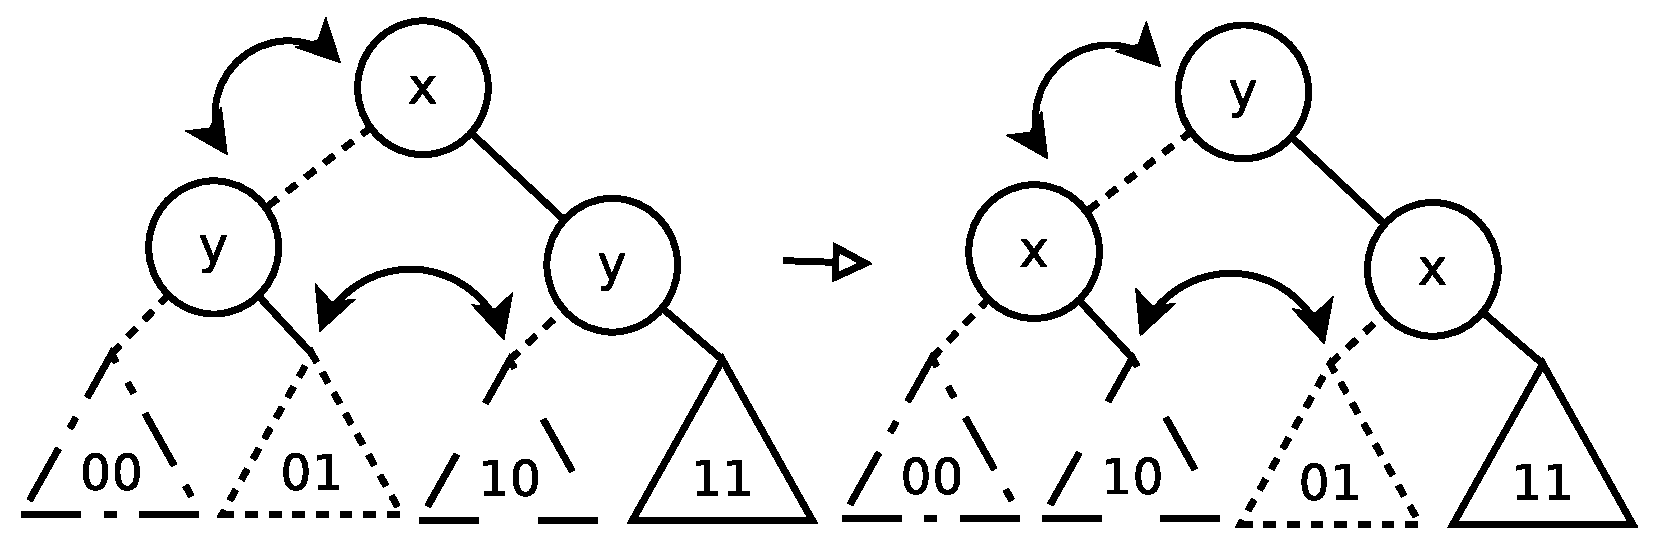
\includegraphics[width=\columnwidth]{DynamicReordering1}
%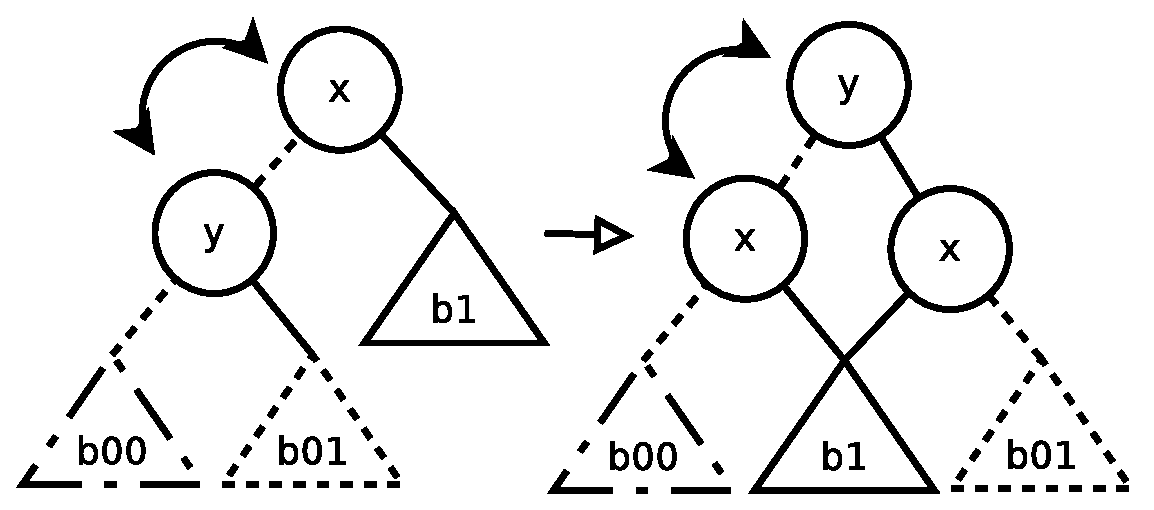
\includegraphics[width=0.9\columnwidth]{DynamicReordering2}
\end{minipage}
}
\savestack{\listingF}{\box0}
\begin{tabular}{|l|l|}
\hline
{\listingB} &
{\listingC} \\ \hline
{\listingD} &
{\listingA} \\ \hline
{\listingE} &
{\listingF} \\ \hline
\end{tabular}

\textbf{Local Model Checking}
\begin{tabular}{|l|l|l|l|}
\hline
\multicolumn{2}{|l|}{\small$\frac{s \vdash_{\Phi} \varphi \wedge \psi}{\{s \vdash_{\Phi} \varphi \} \quad \{s \vdash_{\Phi} \psi\}} \wedge$} & \multicolumn{2}{|l|}{\small$\frac{s \vdash_{\Phi} \varphi \vee \psi}{\{s \vdash_{\Phi} \varphi \} \quad \{s \vdash_{\Phi} \psi\}} \vee $}\\ \hline
\multicolumn{2}{|l|}{\small$\frac{s \vdash_{\Phi} \square \varphi}{\{s_1 \vdash_{\Phi} \varphi\} \dots \{s_n \vdash_{\Phi} \varphi\}} \wedge$}&\multicolumn{2}{|l|}{\small$\frac{s \vdash_{\Phi} \diamondsuit \varphi}{\{s_1 \vdash_{\Phi} \varphi\} \dots \{s_n \vdash_{\Phi} \varphi\}} \vee$} \\
 \hline
\multicolumn{2}{|l|}{\small$\frac{s \vdash_{\Phi} \overleftarrow{\square} \varphi}{\{s'_1 \vdash_{\Phi} \varphi \}\dots \{ s'_n \vdash_{\Phi} \varphi\}} \wedge$} &\multicolumn{2}{|l|}{\small$\frac{s \vdash_{\Phi} \overleftarrow{\diamondsuit} \varphi}{\{s'_1 \vdash_{\Phi} \varphi \}\dots \{ s'_n \vdash_{\Phi} \varphi\}} \vee$} \\
 \hline
$\frac{s \vdash_{\Phi} \mu x.\varphi}{s \vdash_{\Phi} \varphi}$ &$\frac{s \vdash_{\Phi} \nu x.\varphi}{s \vdash_{\Phi} \varphi}$&$\frac{s \vdash_{\Phi} x}{s \vdash_{\Phi} \Db_{\Phi}(x)}$&$\frac{\Db_{\Phi}\text{\tiny (replace w.}}{\text{\tiny initial form.)}}$\\
 \hline
\multicolumn{4}{|l|}{$\{s_1 \dots s_n \}=suc^{\Rb}_{\exists}({s})$ and $\{s'_1 \dots s'_n \}=pre^{\Rb}_{\exists}({s})$}\\ \hline 
\end{tabular}
\textbf{Approximations and Ranks}
\begin{tabular}{|l|l|}
\hline
If (s,$\mu x.\varphi$) repeats$\rightarrow$return 1&$apx_0(\mu x.\varphi):=0$\\ \hline
If (s,$\nu x.\varphi$) repeats$\rightarrow$return 0& $apx_0(\nu x.\varphi):=1$\\ \hline
%\multicolumn{2}{|l|}{$apx_{n+1}(\mu x.\varphi):=[\varphi]_{x}^{apx{n}(\mu x.\varphi)}$}\\ \hline
%\multicolumn{2}{|l|}{$apx_{n+1}(\nu x.\varphi):=[\varphi]_{x}^{apx{n}(\nu x.\varphi)}$}\\ \hline
\end{tabular} \\


\textbf{Tarski-Knaster Theorem}: $\mu := \text{starts} \; \bot \rightarrowtriangle \text{least fixpoint} \;\spadesuit \; \nu :=\text{starts} \;\top \rightarrowtriangle \text{greatest fixpoint}$

%\begin{window}[1, l, 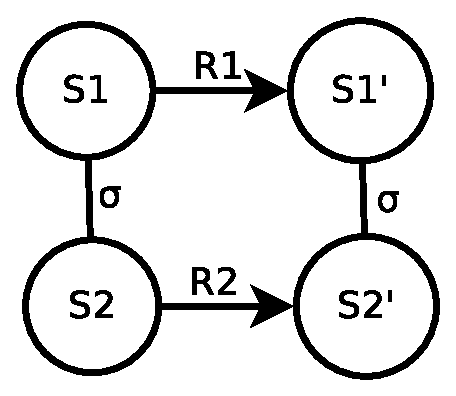
\includegraphics[width=0.3\columnwidth]{Simulation}, {}]
%\textbf{Simulation}: given ${\Kb_{1}=(\Ib_1,\Sb_1,\Rb_1,\Lb_1)}$ and ${\Kb_{2}=(\Ib_2,\Sb_2,\Rb_2,\Lb_2)}$; ${\sigma \subseteq \Sb_1 \times \Sb_2}$ is a sim. relation between $\Kb_1 \text{ and } \Kb_2$ (${\Kb_1 \preccurlyeq \Kb_2}$) if: \textbf{SIM1-} ${(s_1,s_2) \in \sigma}$ implies ${\Lb_1(s_1)=\Lb_2(s_2)}$; \textbf{SIM2-} for $s_1,s'_{1} \in \Sb_1, s_2 \in \Sb_2$ with ${(s_1,s_2) \in \sigma}$ and ${(s_1,s'_{1}) \in \Rb_1}$, there must be ${s'_2 \in \Rb_2}$ with ${(s'_1,s'_2) \in \sigma}$ ${(s_2,s'_{2}) \in \Rb_2}$; \textbf{SIM3-} for all ${s_1 \in \Ib_1}$, there is a ${s_2 \in \Ib_2}$ with ${(s_1,s_2) \in \sigma}$.
%\end{window}
%\textbf{Greatest Simulation Relation}
%${(s_1,s_2) \in \Hb_{0}\Leftrightarrow \Lb_1(s_1)=\Lb_2(s_2)}$

%${(s_1,s_2) \in \Hb_{i+1}\Leftrightarrow}$
%\begin{align*}
%  \begin{pmatrix}
%    (s_1,s_2) \in \Hb_{i} \wedge&\\
%    \forall s'_1 \in \Sb_1.\exists s'_2 \in \Sb_2.&\\
%    (s_1,s'_1) \in \Rb_1 \rightarrow &(s_2,s'_2) \in \Rb_2 \wedge (s'_1,s'_2) \in \Hb_{i}
%  \end{pmatrix}
%\end{align*}
%$\Hb_*$is the greatest simulation relation if \textbf{SIM3}: ${\Ib_1 \subseteq \{s_1 \in \Sb_1 | %\exists s_2 \in \Ib_2 . (s_1, s_2) \in \Hb_* \}}$

%\textbf{Bisimulation}:${\sigma \subseteq \Sb_1 \times \Sb_2}$ is a bisim. relation between $\Kb_1 \text{ and } \Kb_2$ (${\Kb_1 \approx \Kb_2}$) if: \textbf{BISIM1-} ${(s_1,s_2) \in \sigma}$ implies ${\Lb_1(s_1)=\Lb_2(s_2)}$; \textbf{BISIM2a-} $s_1,s'_{1} \in \Sb_1, s_2 \in \Sb_2$, ${(s_1,s_2) \in \sigma}$, ${(s_1,s'_{1}) \in \Rb_1}$, imply that there is ${s'_2 \in \Sb_2}$ with ${(s'_1,s'_2) \in \sigma}$ and ${(s_2,s'_{2}) \in \Rb_2}$;\textbf{BISIM2b-} $s_2,s'_{2} \in \Sb_2, s_1 \in \Sb_1$, ${(s_1,s_2) \in \sigma}$, ${(s_2,s'_{2}) \in \Rb_2}$, imply that there is ${s'_1 \in \Sb_1}$ with ${(s'_1,s'_2) \in \sigma}$ and ${(s_1,s'_{1}) \in \Rb_1}$;\textbf{BISIM3a-} for all ${s_1 \in \Ib_1}$, there is a ${s_2 \in \Ib_2}$ with ${(s_1,s_2) \in \sigma}$;\textbf{BISIM3b-} for all ${s_1 \in \Ib_2}$, there is a ${s_2 \in \Ib_2}$ with ${(s_1,s_2) \in \sigma}$.

%\textbf{Greatest Bisimulation Relation (Equivalence)}
%${(s_1,s_2) \in \Bb_{0}\Leftrightarrow \Lb_1(s_1)=\Lb_2(s_2)}$

%${(s_1,s_2) \in \Bb_{i+1}\Leftrightarrow}$
%\begin{align*}
%  \begin{pmatrix}
%    (s_1,s_2) \in \Bb_{i} \wedge\\
%    \begin{bmatrix}
%    		\forall s'_1 \in \Sb_1.\exists s'_2 \in \Sb_2.\\
%   		(s_1,s'_1) \in \Rb_1 \rightarrow (s_2,s'_2) \in \Rb_2 \wedge (s'_1,s'_2) \in \Bb_{i}
%    \end{bmatrix}\\
%    \begin{bmatrix}
%    		\forall s'_2 \in \Sb_2.\exists s'_1 \in \Sb_1.\\
%   		(s_2,s'_2) \in \Rb_2 \rightarrow (s_1,s'_1) \in \Rb_1 \wedge (s'_1,s'_2) \in \Bb_{i}
%    \end{bmatrix}
%  \end{pmatrix}
%\end{align*}
%$\Bb_*$is the greatest simulation relation if ${\Ib_1 \subseteq \{s_1 \in \Sb_1 | \exists s_2 \in %\Ib_2 . (s_1, s_2) \in \Bb_* \}}$ ${\Ib_2 \subseteq \{s_2 \in \Sb_2 | \exists s_1 \in \Ib_1 . %(s_1, s_2) \in \Bb_* \}}$

%\textbf{Quotient}: Bisimulation with itself\\%given ${\Kb=(\Ib,\Sb,\Rb,\Lb)}$ and the equivalence relation $\sigma \subseteq \Sb \times \Sb$; Quotient structure $\Kb_{/\sigma}=(\widetilde{\Ib},\widetilde{\Sb},\widetilde{\Rb},\widetilde{\Lb})$:
%$\widetilde{\Ib}:=\{\{s' \in \Sb | (s,s') \in \sigma \} | s \in \Ib \}$
%$\widetilde{\Sb}:=\{\{s' \in \Sb | (s,s') \in \sigma \} | s \in \Sb \}$
%$(\widetilde{s}_1,\widetilde{s}_2) \in \Rb :\Leftrightarrow \exists s'_1 \in \widetilde{s}_1. \exists s'_2 \in \widetilde{s}_2.(s'_1,s'_2) \in \Rb$
%$\widetilde{\Lb}( \widetilde{s} ):= \Lb(s)$


%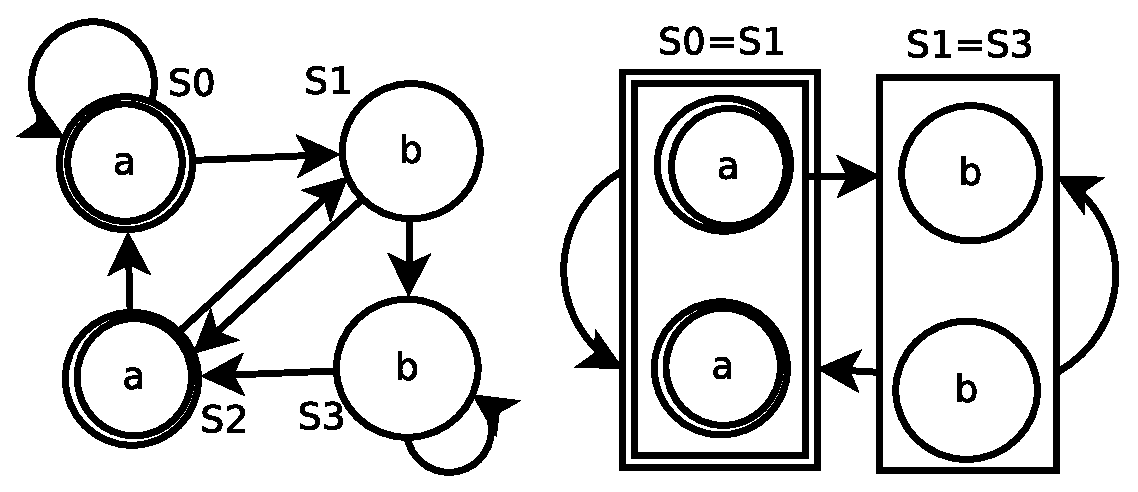
\includegraphics[width=0.7\columnwidth]{Quotient}


%\textbf{Symbolic Product Computation} - given ${\Kb_1=(\Vb_1,\varphi_{\Ib},\varphi_{\Rb})}$ and ${\Kb_2=(\Vb_2,\psi_{\Ib},\psi_{\Rb})}$, the product is: $\Kb_1 \times \Kb_2 = (\Vb_1 \cup \Vb_2, \varphi_{\Ib} \wedge \psi_{\Ib},\varphi_{\Rb} \wedge \psi_{\Rb} )$
\textbf{Quantif.} ${\exists x.\varphi:=[\varphi]^{1}_{x} \vee [\varphi]^{0}_{x}}\; \clubsuit\; {\forall x.\varphi:=[\varphi]^{1}_{x} \wedge [\varphi]^{0}_{x}}$

\textbf{Predecessor and Successor}
$\diamondsuit := pre^{\Rb}_{\exists}(Q) := \exists x'_1,...,x'_n.\varphi_{\Rb} \wedge [\varphi_{Q}]^{x'_1,...,x'_n}_{x_1,...,x_n}$
$\overleftarrow{\diamondsuit} := suc^{\Rb}_{\exists}(Q) := [\exists x_1,...,x_n.\varphi_{\Rb} \wedge \varphi_{Q}]_{x'_1,...,x'_n}^{x_1,...,x_n}$
$\square = pre^{\Rb}_{\forall}(Q) := \forall x'_1,...,x'_n.\varphi_{\Rb} \rightarrow [\varphi_{Q}]^{x'_1,...,x'_n}_{x_1,...,x_n}$
$\overleftarrow{\square} := suc^{\Rb}_{\forall}(Q) := [\forall x_1,...,x_n.\varphi_{\Rb} \rightarrow \varphi_{Q}]_{x'_1,...,x'_n}^{x_1,...,x_n}$
\begin{tabular}{l l}
\raisebox{-0.2\height+\baselineskip}{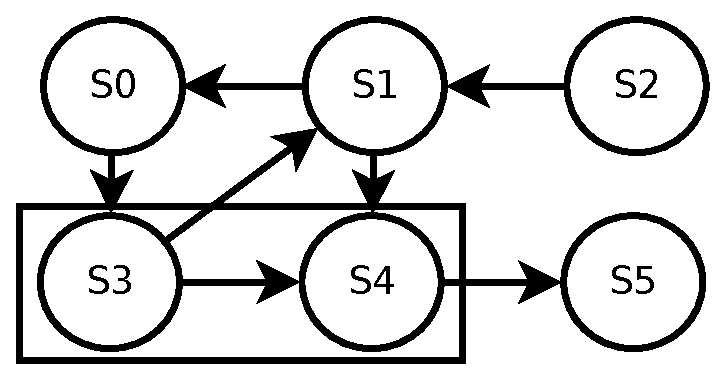
\includegraphics[width=0.33\columnwidth]{universalPre}}
&
{$\!\begin{aligned}
\text{\textbf{Example: }} \square / \overleftarrow{\square} \\
pre_{\forall}^{\Rb}(\{S3,S4\})=\{S0,S5\} \\
suc_{\forall}^{\Rb}(\{S3,S4\})=\{S2,S5\} \\
%pre_{\exists}^{\Rb}(\{S3,S4\})=\{S0,S1,S3\} \\
%suc_{\exists}^{\Rb}(\{S3,S4\})=\{S1,S4,S5\}
\end{aligned}$}
\end{tabular}

\setbox0=\hbox{%
\begin{minipage}{0.425\columnwidth}
% universal predecessor
\begin{lstlisting}[mathescape,style=customc] 
$pre_{\forall}^{\Rb}(Q=\{S_1,...,S_n\})$
for each node n in $\Kb$:
	if(n points to a node that is not in Q)
		n $\notin pre_{\forall}^{\Rb}(Q)$
	else
		n $\in pre_{\forall}^{\Rb}(Q)$
\end{lstlisting}
\end{minipage}
}
\savestack{\listingG}{\box0}
\setbox0=\hbox{%
% universal successor
\begin{minipage}{0.425\columnwidth}
\begin{lstlisting}[mathescape,style={customc}]
$suc_{\forall}^{\Rb}(Q=\{S_1,...,S_n\})$
for each node n in $\Kb$:
	if(n is pointed by a node that is not in Q)
		n $\not\in suc_{\forall}^{\Rb}(Q)$
	else
		n $\in suc_{\forall}^{\Rb}(Q)$
\end{lstlisting}
\end{minipage}
}
\savestack{\listingH}{\box0}

\begin{tabular}{|l|l|}
\hline
{\listingG} &
{\listingH} \\ \hline
\end{tabular}

%%%%%%%%%%%%%%%%%%%%%%%%
%%% If we find something small, we can add it here in this space
%%%%%%%%%%%%%%%%%%%%%%%%
%\vfill
%\columnbreak
%\textbf{\textit{* Rabin-Scott Subset Construction}}
%\textbf{1.} Initial state is a set of states containing all the initial states.
%\textbf{2.} For all transitions of a set of states, compute the successors and create a set of states containing all the possible reachable states when performing that transition.
%\textbf{3.} Acceptance condition are set of states containing acceptance states.
%%%%%%%%%%%%%%%%%%%%%%%%

\textbf{\#\#\#AUTOMATA}

\textbf{Automata types:} G$\rightarrow$Safety; F$\rightarrow$Liveness; FG$\rightarrow$Persistence/Co-Buchi; GF$\rightarrow$Fairness/Buchi.

\textbf{\underline{Automaton Determinization}}\\
\textbf{NDet\textsubscript{G}\textrightarrow Det\textsubscript{G}:} 
1.Remove all states/edges that do not satisfy acceptance condition;
2.Use Subset construction (Rabin-Scott);
3.Acceptance condition will be the states where \{\} is never reached. \\
\textbf{\{NDet\textsubscript{F}(partial) or NDet\textsubscript{prefix}\}\textrightarrow Det\textsubscript{FG}:} 
Breakpoint Construction. \\
\textbf{NDet\textsubscript{F} (total)\textrightarrow Det\textsubscript{F}:}
Subset Construction. \\
\textbf{NDet\textsubscript{FG}\textrightarrow Det\textsubscript{FG}:}
Breakpoint Construction.\\
\textbf{NDet\textsubscript{GF}\textrightarrow \{Det\textsubscript{Rabin} or Det\textsubscript{Streett}\}:}
Safra Algorithm.

%\textbf{\textit{* Rabin-Scott Subset Construction}}
%\textbf{1.} Initial state is a set of states containing all the initial states.
%\textbf{2.} For every possible transition of a set of states, compute the successors and create a set of states containing all the possible reachable states when performing that transition.
%\textbf{3.} Acceptance condition are set of states containing acceptance states.

%\textbf{\textit{* Breakpoint Construction}}
%\textbf{1.} Each state is composed by two components
%\textbf{2.} Initial state first component is a set of all initial states, and second component is the empty set. Ex.: $(\Ib,\{\})$.
%\textbf{3.} a successor for a state (Q,Q\textsubscript{f}) is generated as follows:
%\begin{align*}
%\begin{cases}
%\text{If }Q_f = \{\} & (suc^{\Rb_{a}}_{\exists}(Q), (suc^{\Rb_{a}}_{\exists}(Q) \cap \Fb) \\
%\text{Otherwise} & (suc^{\Rb_{a}}_{\exists}(Q), (suc^{\Rb_{a}}_{\exists}(Q_f) \cap \Fb) \\
%\end{cases}
%\end{align*}
%\textbf{4.} Acceptance states are states where $Q_f \neq \{\}$.

\textbf{Boolean Operations on $\omega$-Automata}
\underline{Complement}
\begin{align*}
\neg \Ab_{\forall}(Q,\Ib,\Rb,\Fb)=\Ab_{\exists}(Q,\Ib,\Rb,\neg \Fb) \\
\neg \Ab_{\exists}(Q,\Ib,\Rb,\Fb)=\Ab_{\forall}(Q,\Ib,\Rb,\neg \Fb)
\end{align*}
\underline{Conjunction}
\begin{align*}
(\Ab_{\exists}(Q_1,\Ib_1,\Rb_1,\Fb_1)\wedge \Ab_{\exists}(Q_2,\Ib_2,\Rb_2,\Fb_2)&)=\\
\Ab_{\exists}(Q_1 \cup Q_2,\Ib_1 \wedge \Ib_2,\Rb_1 \wedge \Rb_2,\Fb_1 \wedge \Fb_2)&
\end{align*}

\underline{Disjunction}
\begin{align*}
(\Ab_{\exists}(Q_1,\Ib_1,\Rb_1,\Fb_1)\vee \Ab_{\exists}(Q_2,\Ib_2,\Rb_2,\Fb_2)&)=\\
\Ab_{\exists} \begin{pmatrix}
Q_1 \cup Q_2 \cup \{q\},\\
(\neg q \wedge \Ib_1) \vee (q \wedge \Ib_2), \\
(\neg q \wedge \Rb_1 \wedge \neg q') \vee ( q \wedge \Rb_2 \wedge q'), \\
(\neg q \wedge \Fb_1) \vee (q \wedge \Fb_2)
  \end{pmatrix}
\end{align*}
\textit{If both automata are totally defined,}
\begin{align*}
(\Ab_{\exists}(Q_1,\Ib_1,\Rb_1,\Fb_1)\vee \Ab_{\exists}(Q_2,\Ib_2,\Rb_2,\Fb_2)&)=\\
\Ab_{\exists}(Q_1 \cup Q_2,\Ib_1 \wedge \Ib_2,\Rb_1 \wedge \Rb_2,\Fb_1 \vee \Fb_2)
\end{align*}
\underline{Eliminate Nesting} - Acceptance condition \textbf{must} be an automata of the same type
\begin{align*}
\Ab_{\exists}(Q^1,\Ib_1^1,\Rb_1^1,\Ab_{\exists}(Q^2,\Ib_1^2,\Rb_1^2,\Fb_1))\\
= \Ab_{\exists}(Q^1 \cup Q^2,\Ib_1^1 \wedge \Ib_1^2,\Rb_1^1 \wedge \Rb_1^2,\Fb_1))
\end{align*}
\underline{Boolean Operations of G}
$(1)\neg G \varphi = F \neg \varphi\qquad \qquad  (2)G \varphi \wedge G \psi = G[\varphi \wedge \psi]$\\
$(3) G \varphi \vee G \psi = \Ab_{\exists}(\{p,q\},p \wedge q,\qquad\qquad$\\
$\qquad\qquad\qquad\qquad[p' \leftrightarrow p \wedge \varphi] \wedge [q' \leftrightarrow q \wedge \psi],G[p \vee q])$\\
%\vfill
%\columnbreak
\underline{Boolean Operations of F}
$(1)\neg F \varphi = G \neg \varphi\qquad \qquad\quad\;(2)F \varphi \vee F \psi = F[\varphi \vee \psi]$\\
$(3) F \varphi \wedge F \psi = \Ab_{\exists}(\{p,q\}, \neg p \wedge \neg q,\qquad\qquad$\\
$\qquad\qquad\qquad\qquad[p' \leftrightarrow p \vee \varphi] \wedge [q' \leftrightarrow q \vee \psi],F[p \wedge q])$
\underline{Boolean Operations of FG}
$(1)\neg FG \varphi = GF \neg \varphi\qquad(2)FG \varphi \wedge FG \psi = FG[\varphi \wedge \psi]$ \\
$(3) FG \varphi \vee FG \psi = \Ab_{\exists}(\{q\}, \neg q, q' \leftrightarrow (q \Rightarrow \psi | \neg \varphi),$\\
$\qquad\qquad\qquad\qquad\qquad FG[\neg q \vee \psi])$\\
\underline{Boolean Operations of GF}
$(1)\neg GF \varphi = FG \neg \varphi \qquad(2)GF \varphi \vee GF \psi = GF[\varphi \vee \psi]$\\
$(3) GF \varphi \wedge GF \psi = \Ab_{\exists}(\{q\}, \neg q, q' \leftrightarrow (q \Rightarrow \neg \psi | \varphi),$\\
$\qquad\qquad\qquad\qquad\qquad GF[q \wedge \psi])$\\
\textbf{Transformation of Acceptance Conditions}
\underline{Reduction of G}\\
$G\varphi = \Ab_{\exists}(\{q\},q,\varphi \wedge q \wedge q',F q))$\\
$G\varphi = \Ab_{\exists}(\{q\},q, q' \leftrightarrow q \wedge \varphi,FG q)$\\
$G\varphi = \Ab_{\exists}(\{q\},q, q' \leftrightarrow q \wedge \varphi,GF q)$\\ 
\underline{Reduction of F}\\
$F\varphi \text{ can \textbf{\underline{not}} be expressed by } NDet_G$\\
$F\varphi = \Ab_{\exists}(\{q\},\neg q, q' \leftrightarrow q \vee \varphi,FG q)$ \\
$F\varphi = \Ab_{\exists}(\{q\},\neg q, q' \leftrightarrow q \vee \varphi,GF q)$\\
\underline{Reduction of FG}
$FG\varphi \text{ can \textbf{\underline{not}} be expressed by } NDet_G$\\
$FG\varphi = \Ab_{\exists}(\{q\},\neg q, q \rightarrow \varphi \wedge q',F q)$\\
$FG\varphi = \Ab_{\exists} \begin{pmatrix}
\{p,q\},\qquad \neg p \wedge \neg q,\\
	\begin{bmatrix}
(p \rightarrow p') \wedge (p' \rightarrow p \vee \neg q) \wedge \\
(q' \leftrightarrow (p \wedge \neg q \vee \neg \varphi) \vee (p \wedge q))
    \end{bmatrix},\\
    G \neg q \wedge F p
\end{pmatrix}$\\
$FG\varphi = \Ab_{\exists} \begin{pmatrix}
\{p,q\},\qquad \neg p \wedge \neg q,\\
	\begin{bmatrix}
(p \rightarrow p') \wedge (p' \rightarrow p \vee \neg q) \wedge \\
(q' \leftrightarrow (p \wedge \neg q \vee \neg \varphi) \vee (p \wedge q))
    \end{bmatrix},\\
    GF[p \wedge \neg q]
\end{pmatrix}$

\textbf{\#\#\#TEMPORAL LOGICS} \\
(S1)Pure LTL: AFGa \\
(S2)LTL + CTL: AFa \\
(S3)Pure CTL: AGEFa \\
(S4)CTL*: AFGa $\vee$ AGEFa \\
\textbf{\underline{Remarks}}
\textit{Beware of Finite Paths}\\
E and A quantify over infinite paths.\\
A$\varphi$ \underline{holds} on every state that has \underline{no infinite path};\\
E$\varphi$ is \underline{false} on every state that has \underline{no infinite path};\\
A0 \underline{holds} on states with \underline{only finite paths};\\
E1 is \underline{false} on state with \underline{only finite paths};\\
$\square$0 holds on states with no successor states;\\
$\diamondsuit$1 holds on states with successor states.\\
$F\varphi = \varphi \vee X F\varphi\qquad\qquad\qquad G\varphi = \varphi \wedge XG \varphi$\\
$[ \varphi \; U\; \psi ] = \psi \vee (\varphi\wedge X[ \varphi \; U\; \psi])$\\
$[ \varphi \; B\; \psi ] = \neg \psi \wedge (\varphi \vee X[ \varphi \; B\; \psi])$\\
$[ \varphi \; W\; \psi] = (\psi \wedge \varphi) \vee (\neg \psi \wedge X[\varphi \; W \; \psi])$

\textbf{LTL Syntactic Sugar:} analog for past operators
$G \varphi = \neg [ 1 \; \underline{U} \; (\neg \varphi)] \qquad \qquad F \varphi = [1\; \underline{U}\; \varphi]$ \\
$[\varphi \; W \;\psi] = \neg [(\neg \varphi \vee \neg \psi)\; \underline{U}\; (\neg \varphi \wedge \psi)]$ \\
$[\varphi \; \underline{W} \;\psi] = [(\neg \psi)\; \underline{U}\; (\varphi \wedge \psi)]$ \tiny\textit{($\neg\psi$ holds until $\varphi \wedge \psi$)}\normalsize \\
$[\varphi \; B \;\psi] = \neg [(\neg \varphi)\; \underline{U}\; \psi)]$ \\
$[\varphi \; \underline{B} \;\psi] = [(\neg \psi)\; \underline{U}\; (\varphi \wedge \neg \psi)]$\tiny\textit{($\psi$ can't hold when $\varphi$ holds)}\normalsize \\
$[\varphi \; U \;\psi] = \neg [(\neg \psi)\; \underline{U}\; (\neg\varphi \wedge \neg \psi)]$\\
$[\varphi \; U \;\psi] = [\varphi \; \underline{U} \;\psi] \vee G \varphi$
$[\varphi \; \underline{U} \;\psi] = \neg [(\neg \psi)\; U\; (\neg \varphi \wedge \neg \psi)]$ \\
$[\varphi \; \underline{U} \;\psi] = \neg [(\neg \psi)\; W\; (\varphi \rightarrow \psi)]$ \\
$[\varphi \; \underline{U} \;\psi] = [\psi\; \underline{W}\; (\varphi \rightarrow \psi)]$ \\
$[\varphi \; \underline{U} \;\psi] = \neg [(\neg \varphi)\; B\; \psi]$\tiny\textit{($\varphi$ doesn't matter when $\psi$ holds)}\normalsize \\
$[\varphi \; \underline{U} \;\psi] = [\psi\; \underline{B}\; (\neg \varphi \wedge \neg \psi]$ \\

\textbf{CTL Syntactic Sugar:} analog for past operators
\underline{Existential Operators}\\
$EF\varphi =  E[1 \; \underline{U} \; \varphi]  $ \\
$EG\varphi =  E[\varphi \; U \; 0]  $ \\
$E[ \varphi \; U \; \psi] =  E[\varphi \; \underline{U}\; \psi] \vee EG\varphi  $ \\
$E[ \varphi \; B \; \psi] =  E[(\neg \psi) \; \underline{U}\; (\varphi \wedge \neg \psi)] \vee EG\neg \psi  $ \\
$E[ \varphi \; B \; \psi] =  E[(\neg \psi) \; U\; (\varphi \wedge \neg \psi)] $ \\
$E[ \varphi \; \underline{B} \; \psi] =  E[(\neg \psi) \; \underline{U}\; (\varphi \wedge \neg \psi)] $ \\
$E[ \varphi \; \underline{B} \; \psi] =  E[(\neg \psi \; \underline{U}\; (\varphi \wedge \neg \psi)] $ \\
$E[ \varphi \; W \; \psi] =  E[(\neg \psi) \; \underline{U}\; (\varphi \wedge \psi)] \vee EG\neg \psi  $ \\
$E[ \varphi \; W \; \psi] =  E[(\neg \psi) \; U\; (\varphi \wedge \psi)] $ \\
$E[ \varphi \; \underline{W} \; \psi] =  E[(\neg \psi) \; \underline{U}\; (\varphi \wedge \psi)] $ \\

\underline{Universal Operators} \\
$AX\varphi =  \neg EX \neg \varphi \qquad$ \\
$AG\varphi=  \neg E[1 \; \underline{U} \; \neg \varphi] $ \\
$AF\varphi =  \neg EG \neg \varphi $ \\
$AF\varphi =  \neg E[(\neg \varphi)\; U\; 0] $ \\
$A[\varphi \; U\; \psi]=  \neg E[(\neg \psi)\; \underline{U} \; (\neg \varphi \wedge \neg \psi)] $ \\
$A[\varphi \; \underline{U} \; \psi] =  \neg E[(\neg \psi) \; \underline{U}\; (\neg \varphi \wedge \neg \psi)]\wedge \neg EG \neg \psi$ \\
$A[\varphi \; \underline{U} \; \psi] =  \neg E[(\neg \psi) \; U\; (\neg \varphi \wedge \neg \psi)]$ \\
$A[\varphi \; B\; \psi]=  \neg E[(\neg \varphi)\; \underline{U} \; \psi] $ \\
$A[\varphi \; \underline{B}\; \psi]=  \neg E[(\neg \varphi)\; U \; \psi] $ \\
$A[\varphi \; \underline{B} \; \psi] =  \neg E[(\neg \varphi \vee \psi) \; \underline{U}\; \psi] \wedge \neg EG(\neg \varphi \vee \psi)$ \\
$A[\varphi \; W\; \psi]=  \neg E[(\neg \psi) \; \underline{U}\; (\neg \varphi \wedge \psi)]$ \\
$A[\varphi \; \underline{W} \; \psi] =  \neg E[(\neg \psi) \; \underline{U}\; (\neg \varphi \wedge \psi)] \wedge \neg EG\neg \psi $ \\
$A[\varphi \; \underline{W} \; \psi] =  \neg E[(\neg \psi) \; U\; (\neg \varphi \wedge \psi)]$\\

\textbf{CTL* to CTL} - \underline{Existential Operators}\\
$EX\varphi = EXE \varphi$\\
$EF\varphi = EFE\varphi\qquad \qquad \qquad EFG\varphi \equiv EFEG\varphi$\\
$E[\varphi\; W \; \psi]=E[(E\varphi)\; W \;\psi]$\\
$E[\varphi\; \underline{W} \; \psi]=E[(E\varphi)\; \underline{W} \;\psi]$\\
$E[\psi\; U \; \varphi]=E[\psi \; U \;E(\varphi)]$\\
$E[\psi\; \underline{U} \; \varphi]=E[\psi \; \underline{U} \;E(\varphi)]$\\
$E[\varphi\; B \; \psi]=E[(E\varphi)\; B \;\psi]$\\
$E[\varphi\; \underline{B} \; \psi]=E[(E\varphi)\; \underline{B} \;\psi]$\\
\textbf{obs.} $EGF\varphi \neq EGEF\varphi \rightarrow$ can't be converted\\ 

\textbf{CTL* to CTL} - \underline{Universal Operators}\\
$AX\varphi = AXA \varphi$\\
$AG\varphi = AGA\varphi$\\
$A[\varphi\; W \; \psi]=A[(A\varphi)\; W \;\psi]$\\
$A[\varphi\; \underline{W} \; \psi]=A[(A\varphi)\; \underline{W} \;\psi]$\\
$A[\varphi\; U \; \psi]=A[A(\varphi) \; U \;\psi]$\\
$A[\varphi\; \underline{U} \; \psi]=A[A(\varphi) \; \underline{U} \;\psi]$\\
$A[\psi\; B \; \varphi]=A[\psi\; B \;(E(\varphi)]$\\
$A[\psi\; \underline{B} \; \varphi]=A[\psi\; \underline{B} \;(E(\varphi)]$\\

\textbf{Weak Equivalences} \\
$*[\varphi U \psi] := [\varphi \underline{U} \psi] \vee G\varphi \ \ \ \ *[\varphi B \psi] := [\varphi \underline{B} \psi] \vee G\neg\psi$ \\
*same to past version$\ \ \ \ \ \ [\varphi W \psi] := \neg[(\neg\varphi) \underline{W} \psi]$ \\
$\overleftarrow{X}\varphi := \neg\overleftarrow{\underline{X}}\neg\varphi\ (at\ t0:\ weak\ true.\ strong\ false) $ \\

\textbf{Negation Normal Form}
${\neg( \varphi \wedge \psi ) = \neg \varphi \vee \neg \psi} \qquad\quad {\neg( \varphi \vee \psi ) = \neg \varphi \wedge \neg \psi }$ \\
${\neg \neg \varphi = \varphi} \qquad\qquad\qquad\qquad  {\neg X \varphi = X \neg \varphi}$ \\
${\neg G \varphi = F \neg \varphi}\qquad\qquad\qquad\;\;{\neg F \varphi = G \neg \varphi}$\\
${\neg[\varphi \; U \;\psi] = [ (\neg \varphi) \;\underline{B}\; \psi ]}\qquad  {\neg[\varphi\; \underline{U}\; \psi] = [ (\neg \varphi)\; B \;\psi ]}$\\
${\neg[\varphi \; B \;\psi] = [ (\neg \varphi) \;\underline{U}\; \psi ]}\qquad  {\neg[\varphi\; \underline{B}\; \psi] = [ (\neg \varphi)\; U\; \psi ]}$\\
${\neg A \varphi = E \neg \varphi} \qquad\qquad\qquad\;\;  {\neg E \varphi = A \neg \varphi}$ \\
${\neg \overleftarrow{X} \varphi = \underline{\overleftarrow{X}} \neg \varphi } \qquad\qquad\qquad  {\neg \underline{\overleftarrow{X}} \varphi = \overleftarrow{X} \neg \varphi }$\\
${\neg \overleftarrow{G} \varphi = \overleftarrow{F} \neg \varphi } \qquad\qquad\qquad {\neg \overleftarrow{F} \varphi = \overleftarrow{G} \neg \varphi }$\\
${\neg[\varphi \;\overleftarrow{U} \;\psi] = [ (\neg \varphi) \;\overleftarrow{\underline{B}}\; \psi ]}\quad\;\; {\neg[\varphi\; \overleftarrow{\underline{U}}\; \psi] = [ (\neg \varphi)\; \overleftarrow{B} \; \psi ]}$\\
${\neg[\varphi \;\overleftarrow{B} \;\psi] = [ (\neg \varphi) \;\overleftarrow{\underline{U}}\; \psi ]}\quad\;\; {\neg[\varphi\; \overleftarrow{\underline{B}}\; \psi] = [ (\neg \varphi)\; \overleftarrow{U} \; \psi ]}$\\

\textbf{Equivalences and Tips} \\
$[\varphi \underline{U} \psi] \equiv \varphi\ don't\ matter\ when\ \psi\ hold $ \\
$[\varphi \underline{B} \psi] \equiv \psi\ can't\ hold\ when\ \varphi\ hold $ \\
$[\varphi \underline{W} \psi] \equiv \neg\psi\ hold\ until\ \varphi\ \wedge\ \psi $ \\
$[\varphi U \psi] \equiv [\varphi \underline{U} \psi] \vee G\varphi$ \\
$[a \underline{U} Fb] \equiv Fb $ \\
$F[a \underline{U} b] \equiv Fb \equiv [Fa \underline{U} Fb] $ \\
$[\varphi B \psi] \equiv [\varphi \underline{B} \psi] \vee G\neg\psi$ \\
$F[a \underline{B} b] \equiv F[a \wedge \neg b] $ \\
$[\varphi W \psi] \equiv \neg[\neg\varphi \underline{W} \psi]$ \\
$AEA \equiv A\ \ \ \ \ \ \ \ \ \ \ \ \bullet GFX \equiv GXF $ \\
$FF\varphi \equiv F\varphi \ \ \ \ \ \ \ \ \ \bullet GG\varphi \equiv G\varphi$\\
$GF\varphi \equiv XGF\varphi\equiv FGF\varphi \equiv GGF\varphi\equiv GFGF\varphi \equiv FGGF\varphi$\\
$FG\varphi\equiv XFG\varphi \equiv FFG\varphi \equiv GFG\varphi \equiv GFFG\varphi \equiv FGFG\varphi$ \\
$GF(x \vee y) \equiv GFx \vee GFy $ \\
$E(\varphi \wedge \psi) \equiv E\varphi \wedge E \psi (in\ general) $ \\
$E(\varphi \vee \psi) \equiv E\varphi \vee E\psi $ \\
$E[(a \underline{U} b) \wedge (c \underline{U} d)] \equiv $ \\
$\ \ \ \ E[(a \wedge c) \underline{U} (b \wedge E(c \underline{U} d) \vee d \wedge E(a \underline{U} b))] $ \\
$AG(\varphi \wedge \psi) \equiv AG\varphi \wedge AG\psi $ \\

\textbf{Eliminate boolean op. after path quantify}\\
$[\varphi_1\; \underline{U}\; \psi_1] \wedge [\varphi_2\; \underline{U}\; \psi_2] =$\\
$\qquad\qquad\qquad\qquad\begin{bmatrix}
  (\varphi_1 \wedge \varphi_2) \; \underline{U} \; 
  	\begin{pmatrix}
  		\psi_1 \wedge [\varphi_2 \; \underline{U} \psi_2] \vee \\
  		\psi_2 \wedge [\varphi_1 \; \underline{U} \psi_1]\;\;\\
	\end{pmatrix}
  \end{bmatrix}$
$[\varphi_1\; \underline{U}\; \psi_1] \wedge [\varphi_2\; U\; \psi_2] =$\\
$\qquad\qquad\qquad\qquad\begin{bmatrix}
  (\varphi_1 \wedge \varphi_2) \; \underline{U} \; 
  	\begin{pmatrix}
  		\psi_1 \wedge [\varphi_2 \; U \psi_2] \vee \\
  		\psi_2 \wedge [\varphi_1 \; \underline{U} \psi_1]\;\;\\
	\end{pmatrix}
  \end{bmatrix}$
$[\varphi_1\; U\; \psi_1] \wedge [\varphi_2\; U\; \psi_2] =$\\
$\qquad\qquad\qquad\qquad\begin{bmatrix}
  (\varphi_1 \wedge \varphi_2) \; \underline{U} \; 
  	\begin{pmatrix}
  		\psi_1 \wedge [\varphi_2 \; U \psi_2] \vee \\
  		\psi_2 \wedge [\varphi_1 \; U \psi_1]\;\;\\
	\end{pmatrix}
  \end{bmatrix}$

\textbf{\#\#\#MONADIC PREDICATE} \\

\textbf{S1S} \\
First order terms are defined as follows: \\
$-0 \in Term _{\sum}^{S1S} $\\
$-{\textit{t} \in V_{\sum} | typ_{\sum}(\textit{t}) = \mathbb{N}} \subseteq Term _{\sum}^{S1S} $ \\
$-SUC(\tau) \in Term _{\sum}^{S1S} if \tau \in Term _{\sum}^{S1S}$ \\
Formulas $\zeta_{S1S}$ are defined as: \\
$-p^{(t)} \in L_{S1S}$ (predicate p at time t)\\
$-\neg\varphi, \varphi \wedge \psi \in L_{S1S}$ \\
$-\exists t. \varphi \in L_{S1S} $ \\
$-\exists p. \varphi \in L_{S1S} $ \\
where: \\
$-\tau \in Term _{\sum}^{S1S} $ \\
$-\varphi, \psi \in \zeta_{S1S} $ \\
$-t \in V_{\sum} \ with \ typ_{\sum}(t) = \mathbb{N}$ \\
$-p \in V_{\sum} \ with \ typ_{\sum}(p) = \mathbb{N} \rightarrow \mathbb{B}$ \\

\textbf{LO2} \\
first order terms are defined as: \\
$-{\textit{t} \in V_{\sum} | typ_{\sum}(\textit{t}) = \mathbb{N}} \subseteq Term _{\sum}^{LO2} $ \\
formulas LO2 are defined as: \\
$-t1 < t2 \in L_{LO2} $ \\
$-p^{(t)} \in L_{LO2}$ \\
$-\neg\varphi, \varphi \wedge \psi \in L_{LO2}$ \\
$-\exists t. \varphi \in L_{LO2} $ \\
$-\exists p. \varphi \in L_{LO2} $ \\
where: \\
$-t, t_{1}, t_{2}\tau \in V_{\sum} \ with \ typ_{\sum}(_{t}) = typ_{\sum}(_{t1}) = typ_{\sum}(t_{t2}) = \mathbb{N} $ \\
$-\varphi, \psi \in \zeta_{LO2} $ \\
$-t \in V_{\sum} \ with \ typ_{\sum}(t) = \mathbb{N}$ \\
$-p \in V_{\sum} \ with \ typ_{\sum}(p) = \mathbb{N} \rightarrow \mathbb{B}$ \\

\textbf{LO2'}
Consider the following set $\zeta_{LO2'}$ of formulas: \\
$-Subset(p,q), Sing(p), and PSUC(p,q) belong to \zeta_{LO2'}$ \\
$-\neg\varphi, \varphi \wedge \psi $ \\
$-\exists p.\varphi$ \\
where
$-\varphi, \psi \in \zeta_{LO2'}$ \\
$-p \in V_{\sum}\ with\ typ_{\sum}(p) = \mathbb{N} \rightarrow \mathbb{B}$ \\
$\zeta_{LO2'}\ has no numeric variables$ \\
numeric variable \textit{t} is replaced by a singleton set $p_{t}$ \\
$\zeta_{LO2'}$ is as expressive as LO2 and S1S \\

\textbf{\#\#\#TRANSLATIONS} \\

\textbf{CTL* Modelchecking to LTL model checking}
Let's $\varphi_i$ be a pure path formula (without path quantifiers), $\Psi$ be a propositional formula, abbreviate subformulas $E\varphi$ and $A\psi$ working bottom-up the syntax tree to obtain the following normal form:
$\upphi = \text{let} \begin{bmatrix}
x_1 = A\varphi_1\\
\vdots \\
x_n = A\varphi_n
\end{bmatrix}
\text{ in } \Psi \text{ end}$\\
Use LTL model checking to compute $Q_i:=\llbracket A\varphi_i\rrbracket _{\Kb_{i-1}}$, where $\Kb_0 := \Kb$ and $\Kb_{i+1}$ is obtained from $\Kb_i$ by labelling the states $Q_i$ with $x_i$.
Finally compute $\llbracket \Psi \rrbracket_{\Kb_n}$

\textbf{function LO2\_S1S($\Phi$)} \\
\ \ \textbf{case $\Phi$ of} \\
$\ \ \ \ t1 < t2 : \textbf{return}\ \exists p. [\forall t. p^{(t)} \rightarrow p^{(SUC(t))} ] \wedge \neg p^{(t1)} \wedge p^{(t2)}:$ \\
$\ \ \ \ p^{(t)} : \textbf{return}\ p^{(t)}; $ \\
$\ \ \ \ \neg \varphi : \textbf{return}\ \neg LO2\_S1S(\varphi); $ \\
$\ \ \ \ \varphi \wedge \psi : \textbf{return}\ LO2\_S1S(\varphi) \wedge LO2\_S1S(\psi); $ \\
$\ \ \ \ \exists t.\varphi : \textbf{return}\ \exists t.LO2\_S1S(\varphi);$ \\
$\ \ \ \ \exists p.\varphi : \textbf{return}\ \exists p.LO2\_S1S(\varphi); $ \\
\ \ \textbf{end} \\
\textbf{end} \\

\textbf{function S1S\_LO2($\Phi$)} \\
\ \ \textbf{case $\Phi$ of} \\
$\ \ \ \ p^{(n)} : \textbf{return}\ \exists t0...tn. p^{(tn)} \wedge zero(t0) \wedge \bigwedge_{i=0}^{n-1} succ(ti, ti + 1); $ \\
$\ \ \ \ p^{(t0 + n)} : \textbf{return}\ \exists t1...tn. p^{(tn)} \wedge \bigwedge_{i=0}^{n-1} succ(ti, ti + 1); $ \\
$\ \ \ \ \neg \varphi : \textbf{return}\ \neg S1S\_LO2(\varphi); $ \\
$\ \ \ \ \varphi \wedge \psi : \textbf{return}\ S1S\_LO2(\varphi) \wedge S1S\_LO2(\psi); $ \\
$\ \ \ \ \exists t.\varphi : \textbf{return}\ \exists t.S1S\_LO2(\varphi);$ \\
$\ \ \ \ \exists p.\varphi : \textbf{return}\ \exists p.S1S\_LO2(\varphi); $ \\
\ \ \textbf{end} \\
\textbf{end} \\

%\textbf{function ElimFO($\Phi$)} (LO2 TO LO2')\\
%\ \ \textbf{case $\Phi$ of} \\
%$\ \ \ \ t1 = t2: \textbf{return}\ Subset(q_{t1}, q_{t2}) \wedge Subset(q_{t2}, q_{t1})$ \\
%$\ \ \ \ t1 < t2: \Psi :\equiv \forall q1. \forall q2.PSUC(q1, q2) \rightarrow [Subset(q1,p) \rightarrow Subset(q2,p)];$ \\
%$\ \ \ \ \ \ \ \ \textbf{return}\ \exists p.\Psi \wedge \neg Subset(qt1, p)\wedge Subset(qt2, p);$ \\
%$\ \ \ \ p^{(t)} : \textbf{return}\ Subset(qt, p)$ \\
%$\ \ \ \ \neg \varphi : \textbf{return}\ \neg ElimFO(\varphi); $ \\
%$\ \ \ \ \varphi \wedge \psi : \textbf{return}\ ElimFO(\varphi) \wedge ElimFO(\psi); $ \\
%$\ \ \ \ \varphi \vee \psi : \textbf{return}\ ElimFO(\varphi) \vee ElimFO(\psi); $ \\
%$\ \ \ \ \exists t.\varphi : \textbf{return}\ \exists qt.Sing(qt)\wedge ElimFO(\varphi);$ \\
%$\ \ \ \ \exists p.\varphi : \textbf{return}\ \exists p.ElimFO(\varphi); $ \\
%\ \ \textbf{end} \\
%\textbf{end} \\

\textbf{function} Tp2Od(t0, $\Phi$) \/\/\textit{temporal to LO1} \\
\ \ \textbf{case $\Phi$ of} \\
\ \ \ \ $is\_var(\Phi): \Psi^{(t0)};$ \\
$\ \ \ \ \neg \varphi : \textbf{return}\ \neg Tp2Od(\varphi); $ \\
$\ \ \ \ \varphi \wedge \psi : \textbf{return}\ Tp2Od(\varphi) \wedge Tp2Od(\psi); $ \\
$\ \ \ \ \varphi \vee \psi : \textbf{return}\ Tp2Od(\varphi) \vee Tp2Od(\psi); $ \\
$\ \ \ \ X\varphi : \Psi := \exists t1.(t0 < t1)\wedge$\\
$\ \ \ \ \ \ \ \ \ \ \ \ \ \ \ \ \forall t2.t0 < t2 \rightarrow t1 \leq t2) \wedge Tp2Od(t1, \varphi);$ \\
$\ \ \ \ [\varphi \underline{U} \psi] : \Psi := \exists t1.t0 \leq t1 \wedge Tp2Od(t1, \psi)\wedge$ \\
$\ \ \ \ \ \ \ \ \ \ \ \ \ \ \ \ \ \ \ \ \ interval((t0, 1, t1, 0), \varphi);$\\
$\ \ \ \ [\varphi B \psi] : \Psi := \forall t1.t0 \leq t1 \wedge $ \\
$\ \ \ \ \ \ \ \ \ \ interval((t0, 1, t1, 0), \neg\varphi) \rightarrow Tp2Od(t1, \neg\psi);$\\
$\ \ \ \ \overleftarrow{X}\varphi : \Psi := \forall t1.(t1 < t0)\wedge$ \\
$\ \ \ \ \ \ \ \ \ \ \ \ \ \ \ \ (\forall t2.t2 < t0 \rightarrow t2 \leq t1) \rightarrow Tp2Od(t1, \varphi);$ \\
$\ \ \ \ \overleftarrow{\underline{X}}\varphi : \Psi := \exists t1.(t1 < t0)\wedge$ \\
$\ \ \ \ \ \ \ \ \ \ \ \ \ \ \ \ (\forall t2.t2 < t0 \rightarrow t2 \leq t1) \wedge Tp2Od(t1, \varphi);$ \\
$\ \ \ \ [\varphi \overleftarrow{\underline{U}} \psi] : \Psi := \exists t1.t1 \leq t0 \wedge Tp2Od(t1, \psi)\wedge$ \\
$\ \ \ \ \ \ \ \ \ \ \ \ \ \ \ \ interval((t1, 0, t0, 1), \varphi);$\\
$\ \ \ \ [\varphi \overleftarrow{B} \psi] : \Psi := \forall t1.t1 \leq t0 \wedge$ \\
$\ \ \ \ \ \ \ \ \ \ \ \ \ \ \ \ interval((t1, 0, t0, 1), \neg\varphi) \rightarrow Tp2Od(t1, \neg\psi);$\\
\ \ \textbf{end} \\
\ \ \textbf{return}\ $\Psi$ \\
\textbf{end} \\

\textbf{function} interval(l, $\varphi$)\\
\ \ \textbf{case $\Phi$ of} \\
$\ \ \ (t0, 0, t1, 0) : $ \\
$\ \ \ \ \ \ \textbf{return}\ \forall t2.t0 < t2 \wedge t2 < t1 \rightarrow Tp2Od(t2, \varphi);$ \\
$\ \ \ (t0, 0, t1, 1) : $ \\
$\ \ \ \ \ \ \textbf{return}\ \forall t2.t0 < t2 \wedge t2 \leq t1 \rightarrow Tp2Od(t2, \varphi);$ \\
$\ \ \ (t0, 1, t1, 0) :$ \\
$\ \ \ \ \ \ \textbf{return}\ \forall t2.t0 \leq t2 \wedge t2 < t1 \rightarrow Tp2Od(t2, \varphi);$ \\
$\ \ \ (t0, 1, t1, 1) :$ \\
$\ \ \ \ \ \ \textbf{return}\ \forall t2.t0 \leq t2 \wedge t2 \leq3 t1 \rightarrow Tp2Od(t2, \varphi);$ \\
\ \ \textbf{end} \\
\textbf{end} \\

\textbf{$\omega$-Automaton to LO2} \\
$A_{\exists}({q1,...,qn}, \psi I, \psi R, \psi F) \textit{(input automaton)}$ \\
$\exists q1..qn, \Theta LO2(0,\psi I) \wedge (\forall t.\Theta LO2(t,\psi R)) \wedge (\forall.t1\exists t2. t1 < t2 \wedge \Theta LO2(t2,\psi F))$ \\
\textbf{Where $\Theta$LO2(t, $\Phi$) is:} \\
-$\Theta LO2(t, p) := p(t)\ for\ variable\ p $ \\
-$\Theta LO2(t, X\psi) := \Theta LO2(t+1, \psi)$ \\
-$\Theta LO2(t, \neg\psi) := \neg\Theta LO2(t, \psi)$ \\
-$\Theta LO2(t, \varphi\wedge\psi) := \Theta LO2(t, \varphi) \wedge \Theta LO2(t, \psi)$ \\
-$\Theta LO2(t, \varphi\vee\psi) := \Theta LO2(t, \varphi) \vee \Theta LO2(t, \psi)$ \\

\textbf{LTL to $\omega$-automata}
% Normal operator
$\upphi \langle X \varphi\rangle_x \Leftrightarrow \Ab_\exists (\{q\},1,q \leftrightarrow X \varphi, \upphi \langle q \rangle_x)$\\
$\upphi \langle X \varphi\rangle_x \Leftrightarrow $ \\
$\ \ \ \ \Ab_\exists (\{q_0,q_1\},1,(q_0 \leftrightarrow \varphi) \wedge (q_1 \leftrightarrow X q_0), \upphi \langle q_1 \rangle_x)$ \\
$\upphi \langle G \varphi\rangle_x \Leftrightarrow $ \\
$\ \ \ \ \Ab_\exists (\{q\},1,q \leftrightarrow \varphi \wedge X q,\upphi \langle q \rangle_x \wedge GF[\varphi \rightarrow q])$ \\
$\upphi \langle F \varphi\rangle_x \Leftrightarrow$ \\
$\ \ \ \ \Ab_\exists (\{q\},1,q \leftrightarrow \varphi \wedge X q, \upphi \langle q \rangle_x \wedge GF[q \rightarrow \varphi])$ \\
$\upphi \langle [\varphi\; U \; \psi] \rangle_x \Leftrightarrow$ \\
$\ \ \ \ \Ab_\exists (\{q\},1,q \leftrightarrow \psi \vee \varphi \wedge X q, \upphi \langle q \rangle_x \wedge GF[\varphi \rightarrow q])$ \\
$\upphi \langle [\varphi\; \underline{U} \; \psi] \rangle_x \Leftrightarrow$ \\
$\ \ \ \ \Ab_\exists (\{q\},1,q \leftrightarrow \psi \vee \varphi \wedge X q, \upphi \langle q \rangle_x \wedge GF[q \rightarrow \psi])$ \\
$\upphi \langle [\varphi\; B \; \psi] \rangle_x \Leftrightarrow$ \\
$\ \ \ \ \Ab_\exists (\{q\},1,q \leftrightarrow \neg\psi \wedge (\varphi \vee X q), \upphi \langle q \rangle_x \wedge GF[q \vee \psi])$ \\
$\upphi \langle [\varphi\; \underline{B} \; \psi] \rangle_x \Leftrightarrow$ \\
$\ \ \ \ \Ab_\exists (\{q\},1,q \leftrightarrow \neg\psi \wedge (\varphi \vee X q), \upphi \langle q \rangle_x \wedge GF[q \rightarrow \varphi])$ \\
% Past operators
$\upphi \langle \overleftarrow{X} \varphi\rangle_x \Leftrightarrow \Ab_\exists (\{q\},q, Xq \leftrightarrow \varphi, \upphi \langle q \rangle_x)$\\
$\upphi \langle \overleftarrow{X} \varphi\rangle_x \Leftrightarrow \Ab_\exists (\{q\},\neg q, Xq \leftrightarrow \varphi, \upphi \langle q \rangle_x)$\\
$\upphi \langle \overleftarrow{G}\varphi\rangle_x \Leftrightarrow \Ab_\exists (\{q\},q, X q \leftrightarrow \varphi \wedge q,\upphi \langle \varphi \wedge q \rangle_x)$
$\upphi \langle \overleftarrow{F}\varphi\rangle_x \Leftrightarrow \Ab_\exists (\{q\},\neg q, X q \leftrightarrow \varphi \vee q,\upphi \langle \varphi \vee q \rangle_x)$
$\upphi \langle [\varphi \; \overleftarrow{U} \; \psi] \rangle_x \Leftrightarrow$ \\
$\ \ \ \ \Ab_\exists (\{q\},q, X q \leftrightarrow \psi \vee \varphi \wedge q, \upphi \langle \psi \vee \varphi \wedge q \rangle_x)$ \\
$\upphi \langle [\varphi \; \overleftarrow{\underline{U}} \; \psi] \rangle_x \Leftrightarrow$ \\ $\ \ \ \ \Ab_\exists (\{q\},\neg q, X q \leftrightarrow \psi \vee \varphi \wedge q, \upphi \langle \psi \vee \varphi \wedge q \rangle_x)$ \\
$\upphi \langle [\varphi\;\overleftarrow{B} \; \psi] \rangle_x \Leftrightarrow$ \\
$\ \ \ \ \Ab_\exists (\{q\},q, X q \leftrightarrow \neg\psi \wedge (\varphi \vee q), \upphi \langle \neg \psi \wedge (\varphi \vee q) \rangle_x)$ \\
$\upphi \langle [\varphi\;\underline{\overleftarrow{B}} \; \psi] \rangle_x \Leftrightarrow$ \\ $\ \ \ \ \Ab_\exists (\{q\},\neg q, X q \leftrightarrow \neg\psi \wedge (\varphi \vee q), \upphi \langle \neg \psi \wedge (\varphi \vee q) \rangle_x)$ \\

\textbf{CTL to $\mu -Calculus (\Phi _{inf} = \nu y.\diamondsuit y$)}
$EX\varphi = \diamondsuit (\Phi_{inf} \wedge \varphi)$ \\
$EG\varphi = \nu x.\varphi \wedge \diamondsuit x $ \\
$EF\varphi = \mu x.\Phi_{inf} \wedge \varphi \vee \diamondsuit x  $ \\
$E[ \varphi \underline{U} \psi] = \mu x.(\Phi_{inf} \wedge \psi) \vee \varphi \wedge \diamondsuit x $ \\
$E[ \varphi U \psi] = \nu x.(\Phi_{inf} \wedge \psi) \vee \varphi \wedge \diamondsuit x $ \\
$E[ \varphi \underline{B} \psi] = \mu x.\neg\psi \wedge (\Phi_{inf} \wedge \varphi \vee \diamondsuit x) $ \\
$E[ \varphi B \psi] = \nu x.\neg\psi \wedge (\Phi_{inf} \wedge \varphi \vee \diamondsuit x) $ \\
$AX\varphi = \square (\Phi_{inf} \rightarrow \varphi)$ \\
$AG\varphi = \nu x.(\Phi_{inf} \rightarrow \varphi) \wedge \square x $ \\
$AF\varphi = \mu x.\varphi \vee \square x  $ \\
$A[ \varphi \underline{U} \psi] = \mu x. \psi \vee (\Phi_{inf} \rightarrow \varphi) \wedge \square x $ \\
$A[ \varphi U \psi] = \nu x.\psi \vee (\Phi_{inf} \rightarrow \varphi) \wedge \square x $ \\
$A[ \varphi \underline{B} \psi] = \mu x.(\Phi_{inf} \rightarrow \neg\psi) \wedge (\varphi \vee \square x) $ \\
$A[ \varphi B \psi] = \nu x.(\Phi_{inf} \rightarrow \neg\psi) \wedge (\varphi \vee \square x)$\\

\textbf{G and $\mu$-calculus (safety property)} \\
-$[\nu x. \varphi \wedge \diamondsuit x]_{K} $ \\
-Contains states s where an infinite path $\pi$ starts with $\forall t. \pi^{(t)} \in [\varphi]_{K}$ \\
-$\varphi$ holds always on $\pi$ \\
\textbf{F and $\mu$-calculus (liveness property)} \\
-$[\mu x. \varphi \vee \diamondsuit x]_{K} $ \\
-Contains states s where a (possibly finite) path $\pi$ starts with $\exists t. \pi^{(t)} \in [\varphi]_{K}$ \\
-$\varphi$ holds at least once on $\pi$ \\
\textbf{FG and $\mu$-calculus (persistence property)} \\
-$[\mu y.[\nu x. \varphi \wedge \diamondsuit x] \vee \diamondsuit y]_{K} $ \\
-Contains states s where an infinite path $\pi$ starts with $\exists t1.\forall t2. \pi^{(t1+t2)} \in [\varphi]_{K}$ \\
-$\varphi$ holds after some point on $\pi$ \\
\textbf{GF and $\mu$-calculus (fairness property)} \\
-$[\nu y.[\mu x. (y \wedge \varphi) \vee \diamondsuit x]]_{K} $ \\
-Contains states s where an infinite path $\pi$ starts with $\forall t1.\exists t2. \pi^{(t1+t2)} \in [\varphi]_{K} ?????t1+t2 or t1+t0?????$ \\
-$\varphi$ holds infinitely often on $\pi$ \\

\end{multicols}
\end{document}
